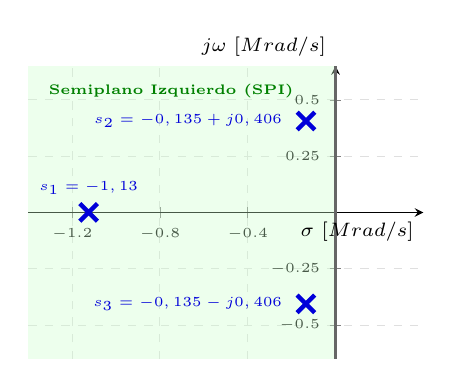
\begin{tikzpicture}
  \begin{axis}[
    width=6.6cm, height=5.3cm,
    axis lines=middle,
    xlabel={$\sigma$ [$\text{Mrad/s}$]},
    ylabel={$j\omega$ [$\text{Mrad/s}$]},
    xlabel style={at={(ticklabel* cs:1)}, anchor=north east, font=\scriptsize},
    ylabel style={at={(ticklabel* cs:1)}, anchor=south east, font=\scriptsize},
    xmin=-1.4, xmax=0.4, ymin=-0.65, ymax=0.65,
    xtick={-1.2, -0.8, -0.4, 0},
    ytick={-0.5, -0.25, 0.25, 0.5},
    grid=both, grid style={gray!25, dashed},
    tick label style={font=\tiny},
  ]
    % Zona estable LHP sombreada
    \fill[green!20, opacity=0.35] (axis cs:-1.4,-0.65) rectangle (axis cs:0,0.65);

    % Eje jw (frontera)
    \draw[line width=1.0pt, black!60] (axis cs:0,-0.65) -- (axis cs:0,0.65);

    % Polo real LHP
    \addplot[only marks, mark=x, mark size=4.5pt, line width=1.6pt, blue!85!black]
      coordinates {(-1.125, 0)};
    \node[above=3pt, blue!85!black, font=\tiny\bfseries, anchor=south] at (axis cs:-1.125, 0) {$s_1 = -1,13$};

    % Polos complejos LHP (estables)
    \addplot[only marks, mark=x, mark size=4.5pt, line width=1.6pt, blue!85!black]
      coordinates {(-0.135, 0.406) (-0.135, -0.406)};
    \node[blue!85!black, font=\tiny\bfseries, anchor=east] at (axis cs:-0.20, 0.406) {$s_{2} = -0,135 + j0,406$};
    \node[blue!85!black, font=\tiny\bfseries, anchor=east] at (axis cs:-0.20, -0.406) {$s_{3} = -0,135 - j0,406$};

    \node[green!50!black, font=\tiny\bfseries, anchor=west] at (axis cs:-1.35, 0.54) {Semiplano Izquierdo (SPI)};
  \end{axis}
\end{tikzpicture}
